
%% ============================================================
%% PŘÍKLAD 5E
%% ============================================================
\section{Příklad 5E -- Časový průběh napětí ve vrubech}

\subsection{Zadání}

Rotační hřídel se dvěma zápichy, axiálně zatížená střídavou silou s~obdélníkovým časovým průběhem.

\textbf{Geometrie} (z~výkresu, celková délka $L_{\mathrm{tot}} = 820\unit{mm}$):
\begin{itemize}[nosep]
    \item Hlavní průměr $D = 50\unit{mm}$, průměr v~zápichu $d = 35\unit{mm}$
    \item Poloměr zápichu $r = 5\unit{mm}$, šířka zápichu $10\unit{mm}$
    \item Úseky: $200 + 10 + 400 + 10 + 200\unit{mm}$
    \item Síla působí v~$x_F = 500\unit{mm}$ od levého vetknutí
    \item Levý vrub: $x \in [200; 210]\unit{mm}$ (před silou)
    \item Pravý vrub: $x \in [610; 620]\unit{mm}$ (za silou)
\end{itemize}

\textbf{Uložení:}
\begin{itemize}[nosep]
    \item \textbf{Vlevo:} pevné vetknutí
    \item \textbf{Vpravo:} jednostranný kontakt s~tuhou stěnou ($\delta = 0$). Posuv do stěny nemožný, od stěny volný — pravá podpora přenáší pouze tlak.
\end{itemize}

\textbf{Zatížení:} obdélníková střídavá osová síla $F = \pm 1{,}4\cdot 10^5\unit{N}$, tolerance velikosti síly $+1000/-0\unit{N}$. Tolerance geometrie $\pm 0{,}5\unit{mm}$ na všech rozměrech.

\textbf{Cíl:} stanovit časový průběh lokálního napětí v~obou vrubech (statický výpočet, $K_t$).

\begin{figure}[H]
\centering
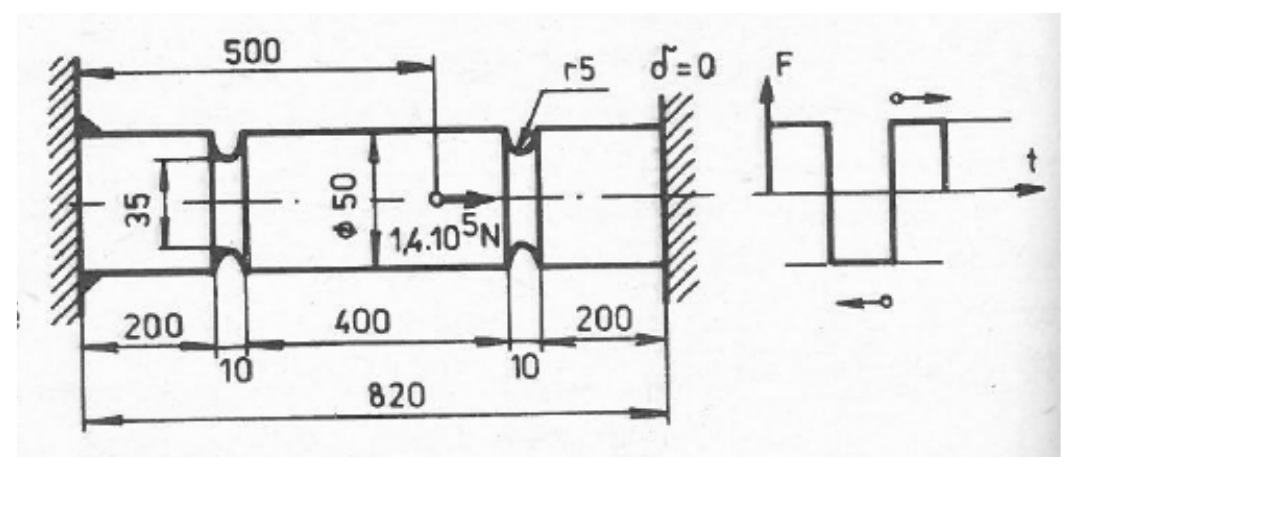
\includegraphics[width=0.85\textwidth]{priklad_5E_zadani.png}
\caption{Zadání: rotační hřídel se dvěma zápichy a~jednostranným kontaktem vpravo, F~$=\pm 1{,}4\E{5}\unit{N}$.}
\end{figure}

\subsection{Deterministické řešení}

\subsubsection{Stav A — staticky neurčitá úloha}

Konvence: tah $+x$ doprava. Označme $R_R$ reakci od pravé stěny (působí v~$-x$, tedy $R_R \le 0$).

Z pravé části hřídele plyne vnitřní osová síla:
\begin{align}
    N_{\mathrm{levá}}(x < x_F) &= F + R_R \\
    N_{\mathrm{pravá}}(x > x_F) &= R_R
\end{align}

\textbf{Podmínka kompatibility} (pravý konec se nepohne, $\Delta_{\mathrm{tot}} = 0$):
\begin{equation}
    N_{\mathrm{levá}} \cdot C_L + N_{\mathrm{pravá}} \cdot C_R = 0
\end{equation}
kde $C_L$, $C_R$ jsou osové poddajnosti levé a~pravé části (násobeno $E$):
\begin{align}
    A_D &= \frac{\pi D^2}{4} = 1963{,}5\unit{mm^2}, \quad A_d = \frac{\pi d^2}{4} = 962{,}1\unit{mm^2} \\
    C_L &= \frac{490}{A_D} + \frac{10}{A_d} = 0{,}24955 + 0{,}01039 = 0{,}25995\unit{mm/mm^2} \\
    C_R &= \frac{310}{A_D} + \frac{10}{A_d} = 0{,}15788 + 0{,}01039 = 0{,}16827\unit{mm/mm^2}
\end{align}

Řešení:
\begin{align}
    R_R &= -F \cdot \frac{C_L}{C_L + C_R} = -140000 \cdot \frac{0{,}25995}{0{,}42822} = -84\,985\unit{N} \\
    N_{\mathrm{levá}}^A &= F + R_R = +55\,015\unit{N} \quad \\
    N_{\mathrm{pravá}}^A &= R_R = -84\,985\unit{N} \quad
\end{align}

\subsubsection{Stav B — staticky určitá úloha}

Pravý konec se odlepí, $R_R = 0$. Z~rovnováhy:
\begin{align}
    N_{\mathrm{levá}}^B &= F + 0 = -140\,000\unit{N} \quad \\
    N_{\mathrm{pravá}}^B &= 0
\end{align}

\subsubsection{Součinitel koncentrace napětí}

Geometrické poměry pro Petersonův graf (kruhový hřídel s~U-vrubem, axiální tah):
\begin{equation}
    \frac{D}{d} = 1{,}429, \qquad \frac{r}{d} = 0{,}143 \quad\Rightarrow\quad \boxed{K_t \approx 2{,}10}
\end{equation}

\begin{figure}[H]
\centering
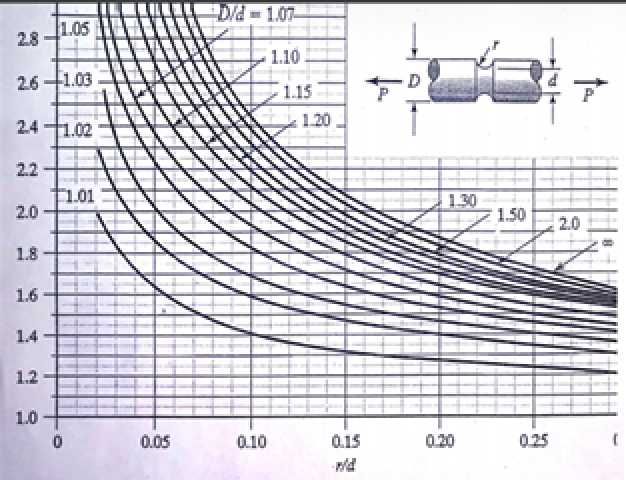
\includegraphics[width=0.5\textwidth]{peterson1.png}
\caption{Petersonův graf pro kruhový hřídel s U vrubem při axiálním tahu}
\end{figure}

(Neuberova aproximace $K_t = 1 + 2\sqrt{t/r} = 3{,}449$ je horní konzervativní mez; Petersonův graf preferován jako přesnější.)

\subsubsection{Lokální napětí ve vrubech}

\textbf{Levý vrub} (v~levé části, působí oba stavy):
\begin{align}
    \sigma_{\mathrm{L}}^A &= K_t \cdot \frac{N_{\mathrm{levá}}^A}{A_d} = 2{,}10 \cdot \frac{55\,015}{962{,}1} = \boxed{+120{,}1\unit{MPa}} \\
    \sigma_{\mathrm{L}}^B &= K_t \cdot \frac{N_{\mathrm{levá}}^B}{A_d} = 2{,}10 \cdot \frac{-140\,000}{962{,}1} = \boxed{-305{,}6\unit{MPa}}
\end{align}

\textbf{Pravý vrub} (v~pravé části, působí jen Stav~A):
\begin{align}
    \sigma_{\mathrm{R}}^A &= K_t \cdot \frac{N_{\mathrm{pravá}}^A}{A_d} = 2{,}10 \cdot \frac{-84\,985}{962{,}1} = \boxed{-185{,}5\unit{MPa}} \\
    \sigma_{\mathrm{R}}^B &= 0\unit{MPa}
\end{align}

\subsection{Časový průběh napětí}

Síla $F(t)$ obdélníkově střídá hodnoty $+140\unit{kN}$ a~$-140\unit{kN}$. Statický výpočet $\Rightarrow$ napětí mezi dvěma diskrétními hodnotami:

\begin{center}
\begin{tabular}{lcccccc}
\toprule
\textbf{Vrub} & $\sigma_{\max}$ & $\sigma_{\min}$ & $\sigma_a$ & $\sigma_m$ & $R = \sigma_{\min}/\sigma_{\max}$ & \textbf{Charakter cyklu} \\
\midrule
Levý  & $+120{,}1$ & $-305{,}6$ & $212{,}8$ & $-92{,}8$ & $-2{,}55$ & asymetrický střídavý \\
Pravý & $0$        & $-185{,}5$ & $92{,}8$  & $-92{,}8$ & $\pm\infty$ & míjivý tlak (0 $\leftrightarrow$ tlak) \\
\bottomrule
\end{tabular}
\end{center}

\subsection{Stochastická analýza}

Rozměry s~tolerancí $\pm 0{,}5\unit{mm}$: $\sigma_{\mathrm{dim}} = 0{,}5/3 \approx 0{,}167\unit{mm}$ (pravidlo $3\sigma$, normální rozdělení). Síla $F \sim \mathcal{U}(140\,000;\,141\,000)\unit{N}$ (uniformní, dle tolerance $+1000/-0$). Náhodné: $D, d, r$, všech 5 délek úseků, poloha síly $x_F$, velikost síly $F$.

\begin{table}[H]
\centering
\caption{Statistiky napětí v~obou vrubech ($N = 100\,000$)}
\begin{tabular}{lccccc}
\toprule
\textbf{Veličina} & $\boldsymbol{\mu}$ & $\boldsymbol{\sigma}$ & \textbf{CoV} & \textbf{95\% CI} \\
\midrule
$\sigma_{\mathrm{L,max}}$ [MPa] & $+120{,}54$ & $1{,}91$ & $0{,}016$ & $[+116{,}85;\; +124{,}33]$ \\
$\sigma_{\mathrm{L,min}}$ [MPa] & $-306{,}74$ & $4{,}80$ & $0{,}016$ & $[-316{,}32;\; -297{,}44]$ \\
$\sigma_{\mathrm{L},a}$    [MPa] & $+213{,}64$ & $3{,}35$ & $0{,}016$ & $[+207{,}15;\; +220{,}32]$ \\
$\sigma_{\mathrm{R,min}}$ [MPa] & $-186{,}20$ & $2{,}91$ & $0{,}016$ & $[-192{,}00;\; -180{,}59]$ \\
$\sigma_{\mathrm{R},a}$    [MPa] & $+93{,}10$  & $1{,}45$ & $0{,}016$ & $[+90{,}29;\; +96{,}00]$ \\
$K_t$ [-] & $2{,}100$ & $0{,}020$ & $0{,}010$ & $[2{,}06;\; 2{,}14]$ \\
\bottomrule
\end{tabular}
\end{table}

Variabilita napětí $\mathrm{CoV} \approx 1{,}6\%$ — nízká, dominuje rozptyl $A_d$ (kvadratická závislost na $d$) a~$K_t$ (citlivost na $r$). Rozptyl síly přispívá řádově $0{,}2\%$ (úzká tolerance).

\begin{figure}[H]
\centering
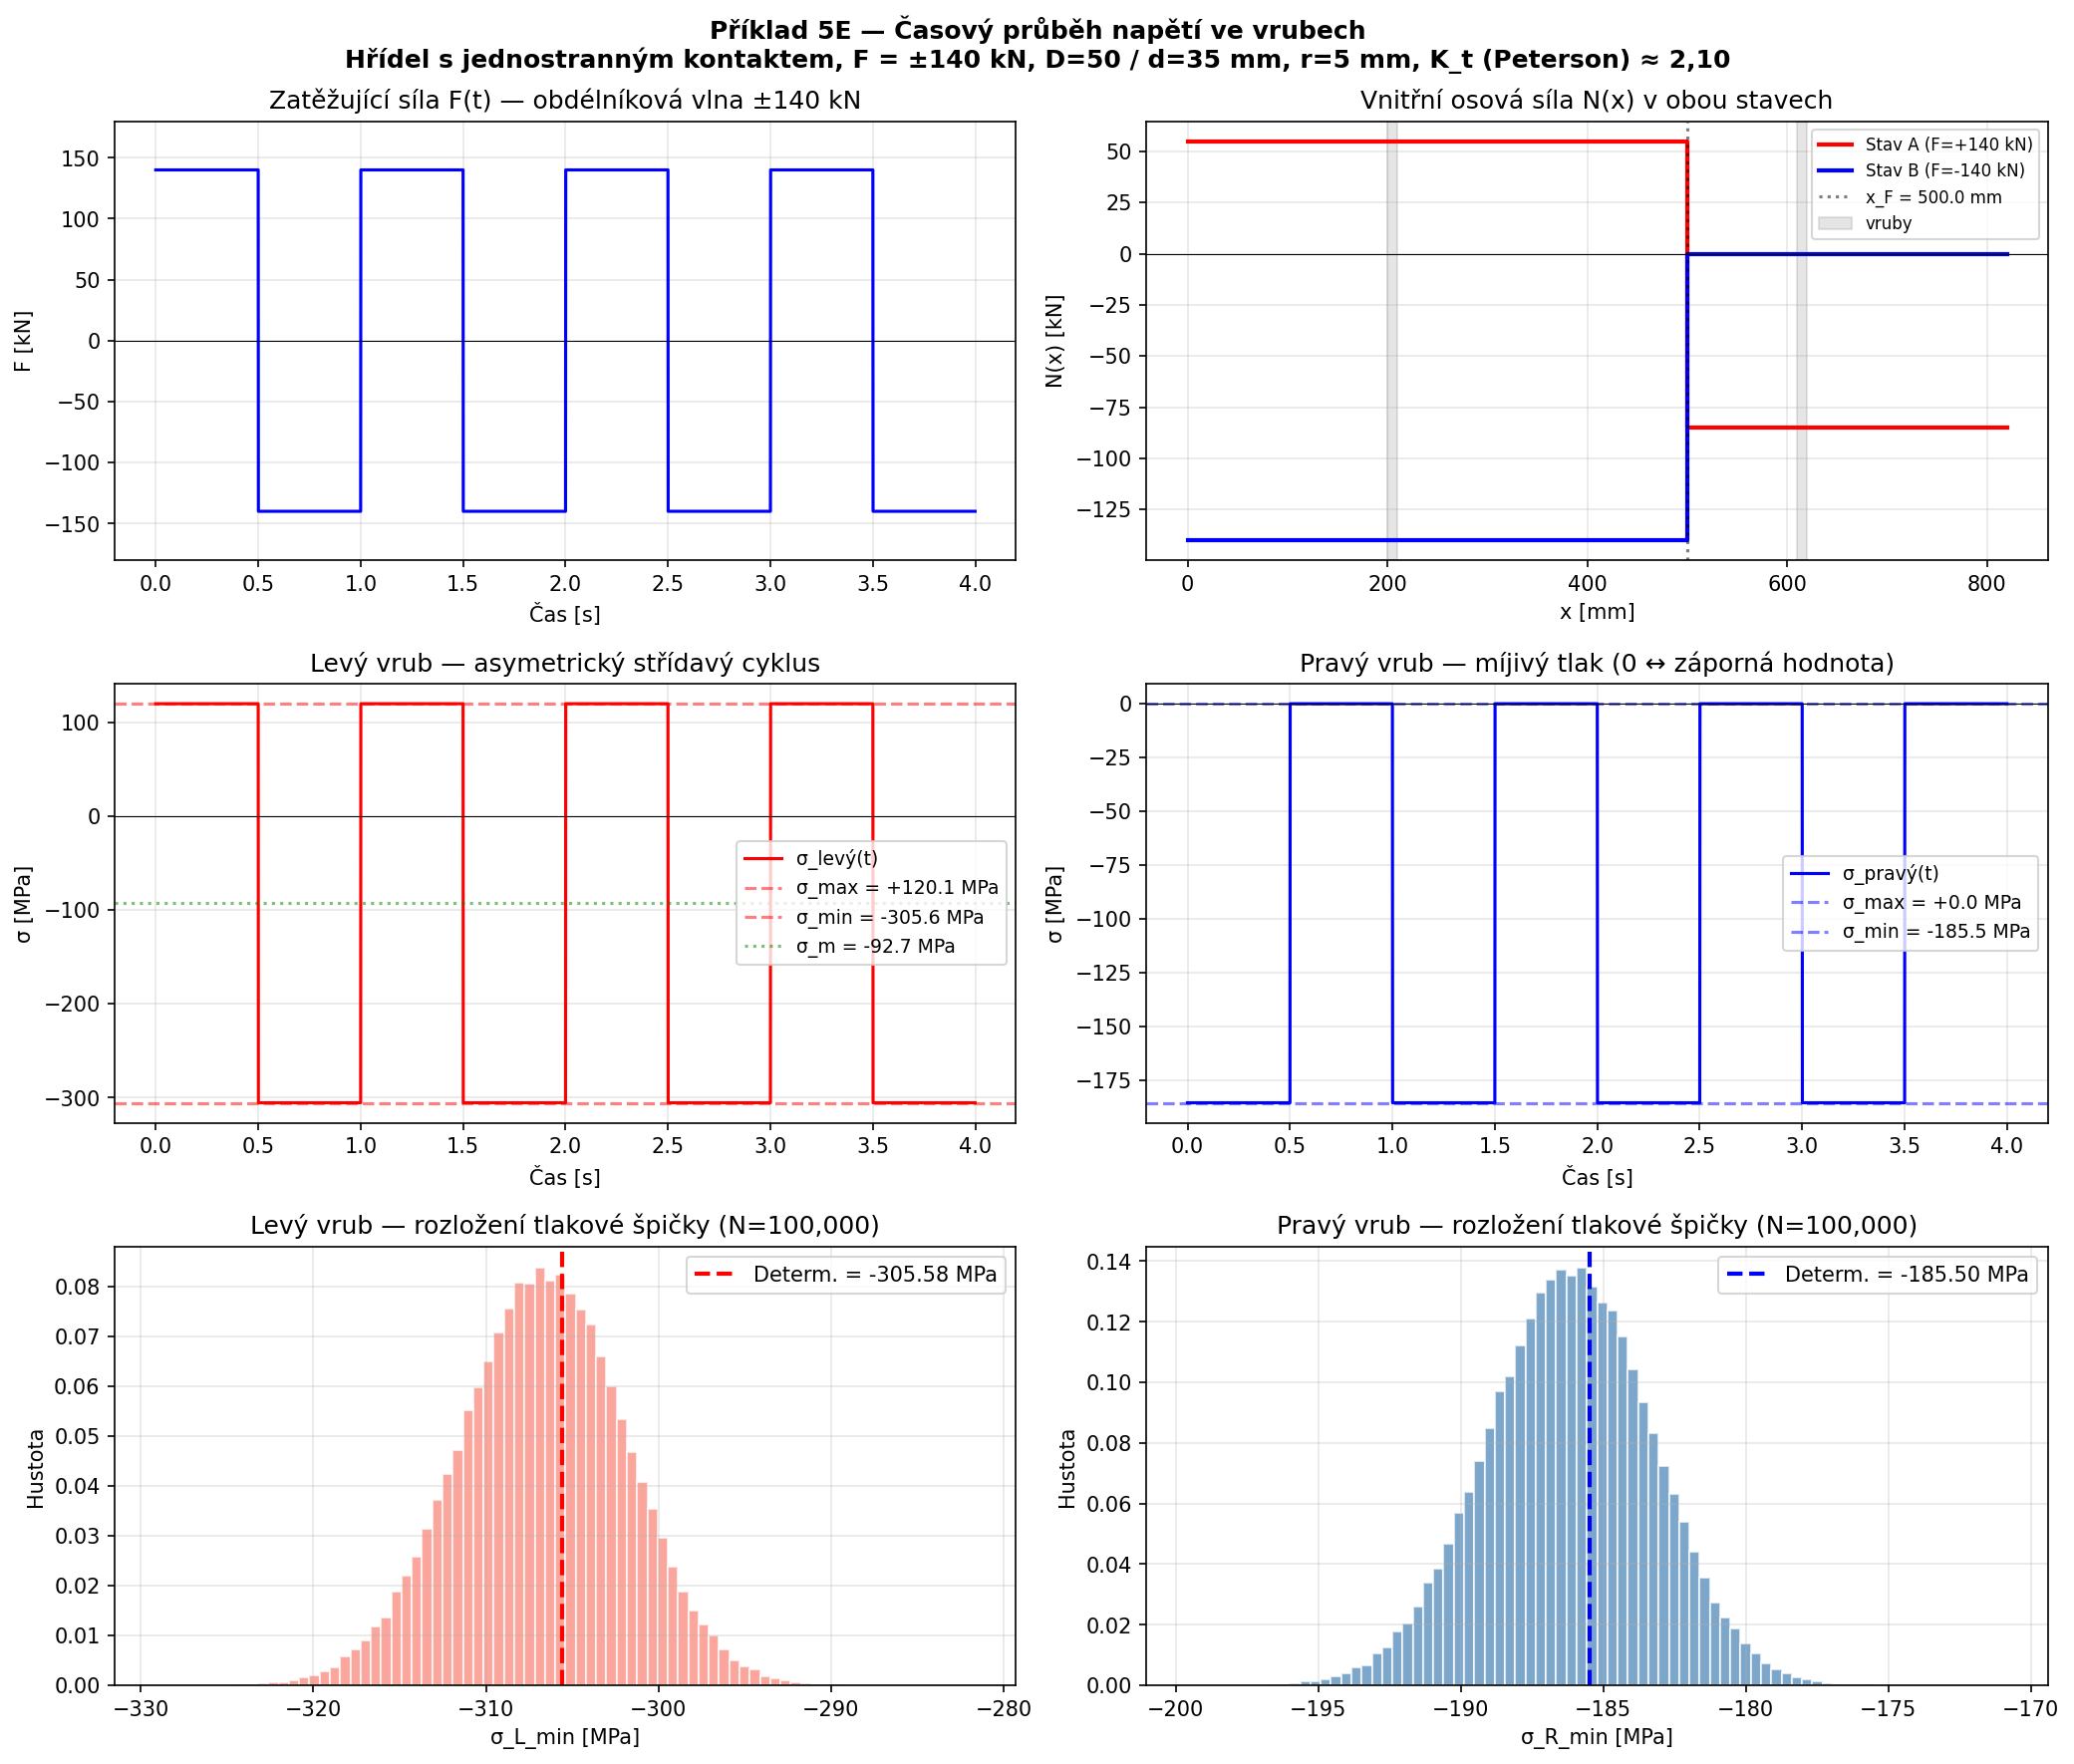
\includegraphics[width=\textwidth]{priklad_5E_vysledky.png}
\caption{Příklad 5E -- Časový průběh síly a~napětí, stochastická analýza}
\label{fig:5E}
\end{figure}

\begin{figure}[H]
\centering
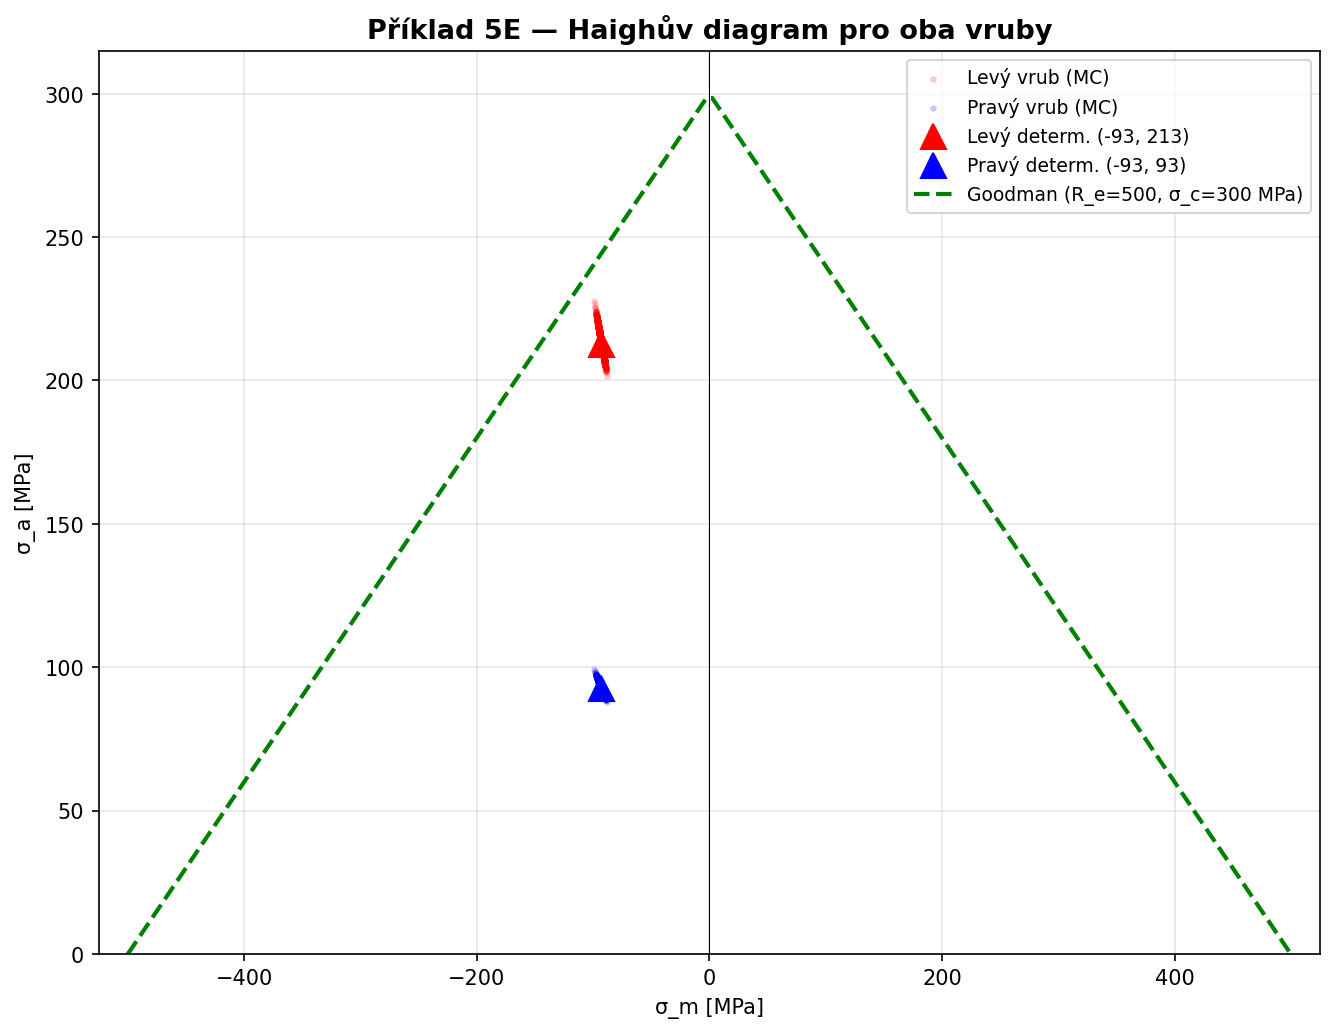
\includegraphics[width=0.5\textwidth]{priklad_5E_haigh.png}
\caption{Příklad 5E -- Haighův diagram ($\sigma_a$ vs $\sigma_m$) s~Goodmanovou přímkou}
\label{fig:5E_haigh}
\end{figure}

